
\documentclass{beamer}
\usepackage{graphicx}

\usepackage[export]{adjustbox}
\usepackage{environ}
\usepackage{calc}
\usepackage{xcolor}

\usepackage{adjustbox}
\usepackage{dashbox}

\newcommand{\cfbox}[2]{%
    \colorlet{currentcolor}{.}%
    {\color{#1}%
    \fbox{\color{currentcolor}#2}}%
}

\usetheme{Boadilla}
\setbeamertemplate{headline}{}
\setbeamertemplate{footline}{}
\setbeamersize{text margin left=0.5cm}
  
\usepackage[english]{babel}
% or whatever

\usepackage[utf8]{inputenc}
% or whatever

\usepackage{times}
\usepackage[T1]{fontenc}
% Or whatever. Note that the encoding and the font should match. If T1
% does not look nice, try deleting the line with the fontenc.



\begin{document}


\begin{frame}{Q: Do species interactions determine diversification?}{}

 %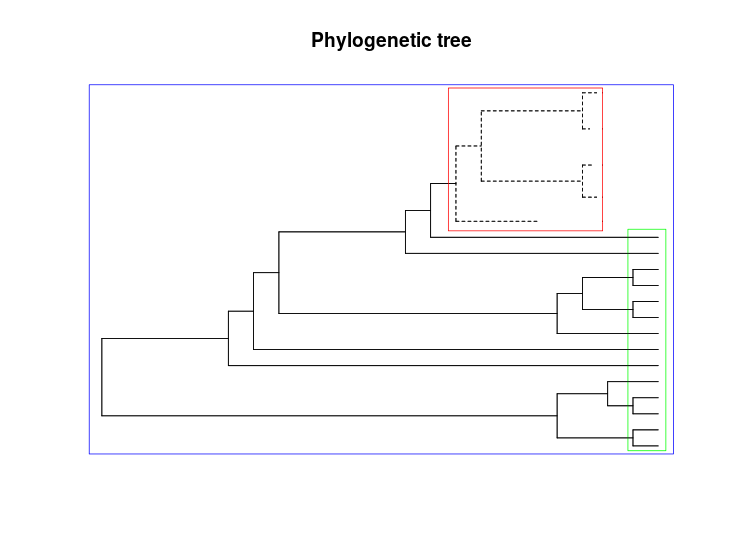
\includegraphics[width=5cm,height=10cm]{phy}


\minipage{0.45\textwidth}
 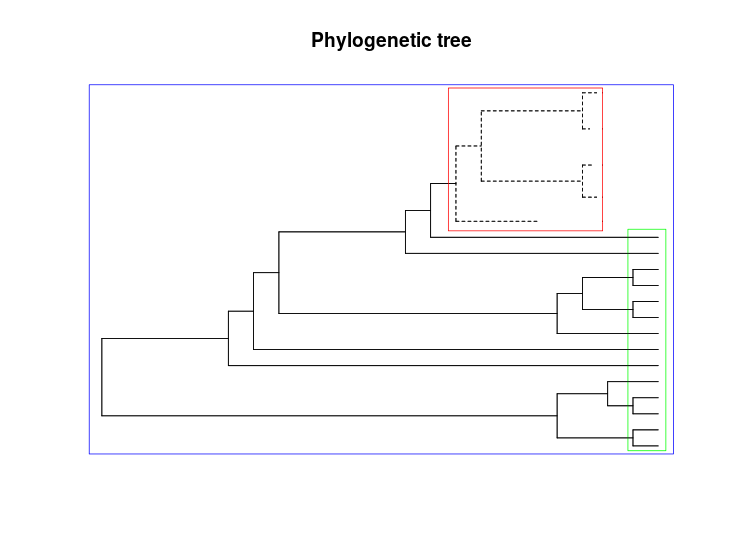
\includegraphics[width=5cm,height=6cm]{phy}
\endminipage
\minipage{0.44\textwidth}
{\tiny
\cfbox{blue}{\parbox{\textwidth}{
{\bf
Problem 1} \\
Model Uncertainly, speciation model.
 }}\\

\cfbox{red}{\parbox{\textwidth}{
{\bf Problem 2}\\
Information on extinct species (fossil record) is absent or, at best, incomplete.

%involve local species interactions, and that such models are really difficult to handle with current methods.
}}\\
\cfbox{green}{\parbox{\textwidth}{
{\bf Problem 3} \\
Models considering local species interaction are computationally unfeasible with current methods.
 }}
}


\endminipage
\\
Approach
\vspace{0.3cm}
%{\scriptsize
\begin{itemize}
{\scriptsize
    \item Inference through data augmentation (solving a hard optimization problem) 
    \item Performing model selection simultaneously. }
\end{itemize}
%}


\end{frame}



\end{document}


